\documentclass[14pt,a4paper]{scrartcl}
\usepackage{cmap}
\usepackage[utf8]{inputenc}
\usepackage[T1,T2A]{fontenc}
\usepackage[english,russian]{babel}
\usepackage{relsize}
\usepackage{graphicx}
\usepackage{subfigure}
\usepackage{mathtools}
\usepackage{amssymb}
\usepackage{float}
\usepackage{sidecap}
\usepackage{wrapfig}
\usepackage{caption}
\usepackage[table,xcdraw]{xcolor}
\usepackage{listings}
\usepackage{amsmath,cryptocode}
\usepackage{listings}
\usepackage{booktabs}
\usepackage{multirow}  
\usepackage{multicol}
\usepackage{bigstrut}
\usepackage{lscape}
\usepackage{rotating}
\usepackage{adjustbox}

\newcommand\scalemath[2]{\scalebox{#1}{\mbox{\ensuremath{\displaystyle #2}}}}


\begin{document}
	\begin{titlepage}
	\begin{center}
		\large
		МИНИСТЕРСТВО ОБРАЗОВАНИЯ И НАУКИ\\ РОССИЙСКОЙ ФЕДЕРАЦИИ
		
		\vspace{0.5cm}
		
		МГТУ им Н.Э.Баумана
		\vspace{0.25cm}
		
		Факультет ФН
		
		Кафедра вычислительной математики и математической физики
		\vfill
		
		
		Соколов Арсений Андреевич\\
		\vfill
		
		
		{\LARGE Лабораторная работа №2 по численным методам\\[2mm]
		}
		\bigskip
		
		3 курс, группа ФН11-53Б\\
		Вариант 9
	\end{center}
	\vfill
	
	\newlength{\ML}
	\settowidth{\ML}{«\underline{\hspace{0.7cm}}» \underline{\hspace{2cm}}}
	\hfill\begin{minipage}{0.4\textwidth}
		Преподаватель\\
		\underline{\hspace{3cm}} В.\,А.~Кутыркин\\
		«\underline{\hspace{0.7cm}}» \underline{\hspace{1.71cm}} 2019 г.
	\end{minipage}%
	\bigskip
	
	
	\vfill
	
	\begin{center}
		Москва, 2019 г.
	\end{center}
\end{titlepage}

\section*{Задание 2.1}
\textbf{Задание.} Дана модель линейной регрессии:
\begin{equation}\label{eq1} 
	Y=x_{*}^{0}+z_{1} x_{*}^{1}+z_{2} x_{*}^{2}+z_{3} x_{*}^{3}+z_{4} x_{*}^{4}+z_{5} x_{*}^{5}+z_{6} x_{*}^{6}+\varepsilon
\end{equation}
Для оценки неизвестных вектора тренда $\prescript{>}{}{x}_* = [x_*^0, \dots, x_*^k \rangle \in \prescript{>}{}{\mathbb{E}}^{k+1}$ и параметра $\sigma$ случайной составляющей $\varepsilon \sim N(0, \sigma)$ модели линейной регрессии \ref{eq1} проводился эксперимент, в котором получены $m=20$ значений $y^1, \dots, y^m \in \mathbb{R}$ регрессора модели \ref{eq1} для $m$ различных наборов $\prescript{>}{}{z}^1 = [z_1^1, \dots, z_6^1 \rangle, \prescript{>}{}{z}^m = [z_1^m, \dots, z_6^m \rangle$ шести факторов модели $\ref{eq1}$.\\
Требуется получить оценки вектора тренда $\prescript{>}{}{x}_* = [x_*^0, \dots, x_*^k \rangle \in \prescript{>}{}{\mathbb{E}}^{k+1}$ и параметра $\sigma$ случайной составляющей $\varepsilon \sim N(0, \sigma)$ модели линейной регрессии \ref{eq1}. Если возможно, редуцировать модель регрессии $\ref{eq1}$ до приведённой модели. Результаты расчётов проиллюстрировать графически, сопроводив необходимыми комментариями.\\
\textbf{Исходные данные.}\\
$N = 9$\\
$\alpha = 1$

\begin{table}[htbp]
	\centering
	\caption{}
	\resizebox{!}{180pt}{
	\begin{tabular}{|rrrrrrr|}
		\hline
		\rowcolor[rgb]{ .357,  .608,  .835} \multicolumn{1}{|c}{\textcolor[rgb]{ 1,  1,  1}{\textbf{Y-a}}} & \multicolumn{1}{c}{\textcolor[rgb]{ 1,  1,  1}{\textbf{z1}}} & \multicolumn{1}{c}{\textcolor[rgb]{ 1,  1,  1}{\textbf{z2}}} & \multicolumn{1}{c}{\textcolor[rgb]{ 1,  1,  1}{\textbf{z3}}} & \multicolumn{1}{c}{\textcolor[rgb]{ 1,  1,  1}{\textbf{z4}}} & \multicolumn{1}{c}{\textcolor[rgb]{ 1,  1,  1}{\textbf{z5}}} & \multicolumn{1}{c|}{\textcolor[rgb]{ 1,  1,  1}{\textbf{z6}}} \bigstrut\\
		\hline
		\rowcolor[rgb]{ .867,  .922,  .969} 13,77 & 1,16  & 1,19  & 1,75  & 1,57  & 1,83  & 1,94 \bigstrut\\
		\hline
		12,41 & 1,24  & 1,91  & 1,18  & 1,04  & 1,30  & 1,92 \bigstrut\\
		\hline
		\rowcolor[rgb]{ .867,  .922,  .969} 12,84 & 1,56  & 1,56  & 1,07  & 1,78  & 1,23  & 1,82 \bigstrut\\
		\hline
		12,60 & 1,74  & 1,80  & 1,95  & 1,75  & 1,25  & 1,55 \bigstrut\\
		\hline
		\rowcolor[rgb]{ .867,  .922,  .969} 12,23 & 1,36  & 1,03  & 1,38  & 1,69  & 1,99  & 1,06 \bigstrut\\
		\hline
		13,88 & 1,54  & 1,74  & 1,58  & 1,06  & 2,00  & 1,43 \bigstrut\\
		\hline
		\rowcolor[rgb]{ .867,  .922,  .969} 14,39 & 1,78  & 1,31  & 1,97  & 1,69  & 1,58  & 1,77 \bigstrut\\
		\hline
		8,56  & 1,14  & 1,14  & 1,69  & 1,22  & 1,03  & 1,02 \bigstrut\\
		\hline
		\rowcolor[rgb]{ .867,  .922,  .969} 9,37  & 1,25  & 1,11  & 1,08  & 1,33  & 1,05  & 1,16 \bigstrut\\
		\hline
		10,95 & 1,42  & 1,35  & 1,68  & 1,00  & 1,47  & 1,10 \bigstrut\\
		\hline
		\rowcolor[rgb]{ .867,  .922,  .969} 13,13 & 1,61  & 1,97  & 1,44  & 1,01  & 1,92  & 1,18 \bigstrut\\
		\hline
		12,83 & 1,52  & 1,43  & 1,46  & 1,01  & 1,11  & 1,98 \bigstrut\\
		\hline
		\rowcolor[rgb]{ .867,  .922,  .969} 11,51 & 1,23  & 1,30  & 1,85  & 1,71  & 1,73  & 1,21 \bigstrut\\
		\hline
		13,90 & 1,73  & 1,87  & 1,07  & 1,10  & 1,98  & 1,26 \bigstrut\\
		\hline
		\rowcolor[rgb]{ .867,  .922,  .969} 14,31 & 1,77  & 1,36  & 1,23  & 1,08  & 1,66  & 1,68 \bigstrut\\
		\hline
		9,67  & 1,42  & 1,07  & 1,12  & 1,44  & 1,06  & 1,08 \bigstrut\\
		\hline
		\rowcolor[rgb]{ .867,  .922,  .969} 11,52 & 1,12  & 1,95  & 1,37  & 1,64  & 1,94  & 1,11 \bigstrut\\
		\hline
		13,18 & 1,73  & 1,80  & 1,37  & 1,18  & 1,12  & 1,88 \bigstrut\\
		\hline
		\rowcolor[rgb]{ .867,  .922,  .969} 12,02 & 1,16  & 1,36  & 1,96  & 1,14  & 1,49  & 1,69 \bigstrut\\
		\hline
		14,16 & 1,96  & 1,27  & 1,25  & 1,19  & 1,47  & 1,62 \bigstrut\\
		\hline
	\end{tabular}}%
	\label{tab:addlabel1}%
\end{table}%

\newpage
\textbf{Решение.}\\
Для получения оценки вектора тренда $\prescript{>}{}{x}_* = [x_*^0, \dots, x_*^k \rangle \in \prescript{>}{}{\mathbb{E}}^{k+1}$ и параметра $\sigma$ случайной составляющей $\varepsilon \sim N(0, \sigma)$ модели линейной регрессии \ref{eq1} воспользуемся программой <<Анализ данных>>, входящей в состав Excel. Переходя на вкладку <<Данные>>, выбираем программу <<анализ данных>>, в которой выбираем пункт <<регрессия>>.
\begin{figure}[h]
	\center{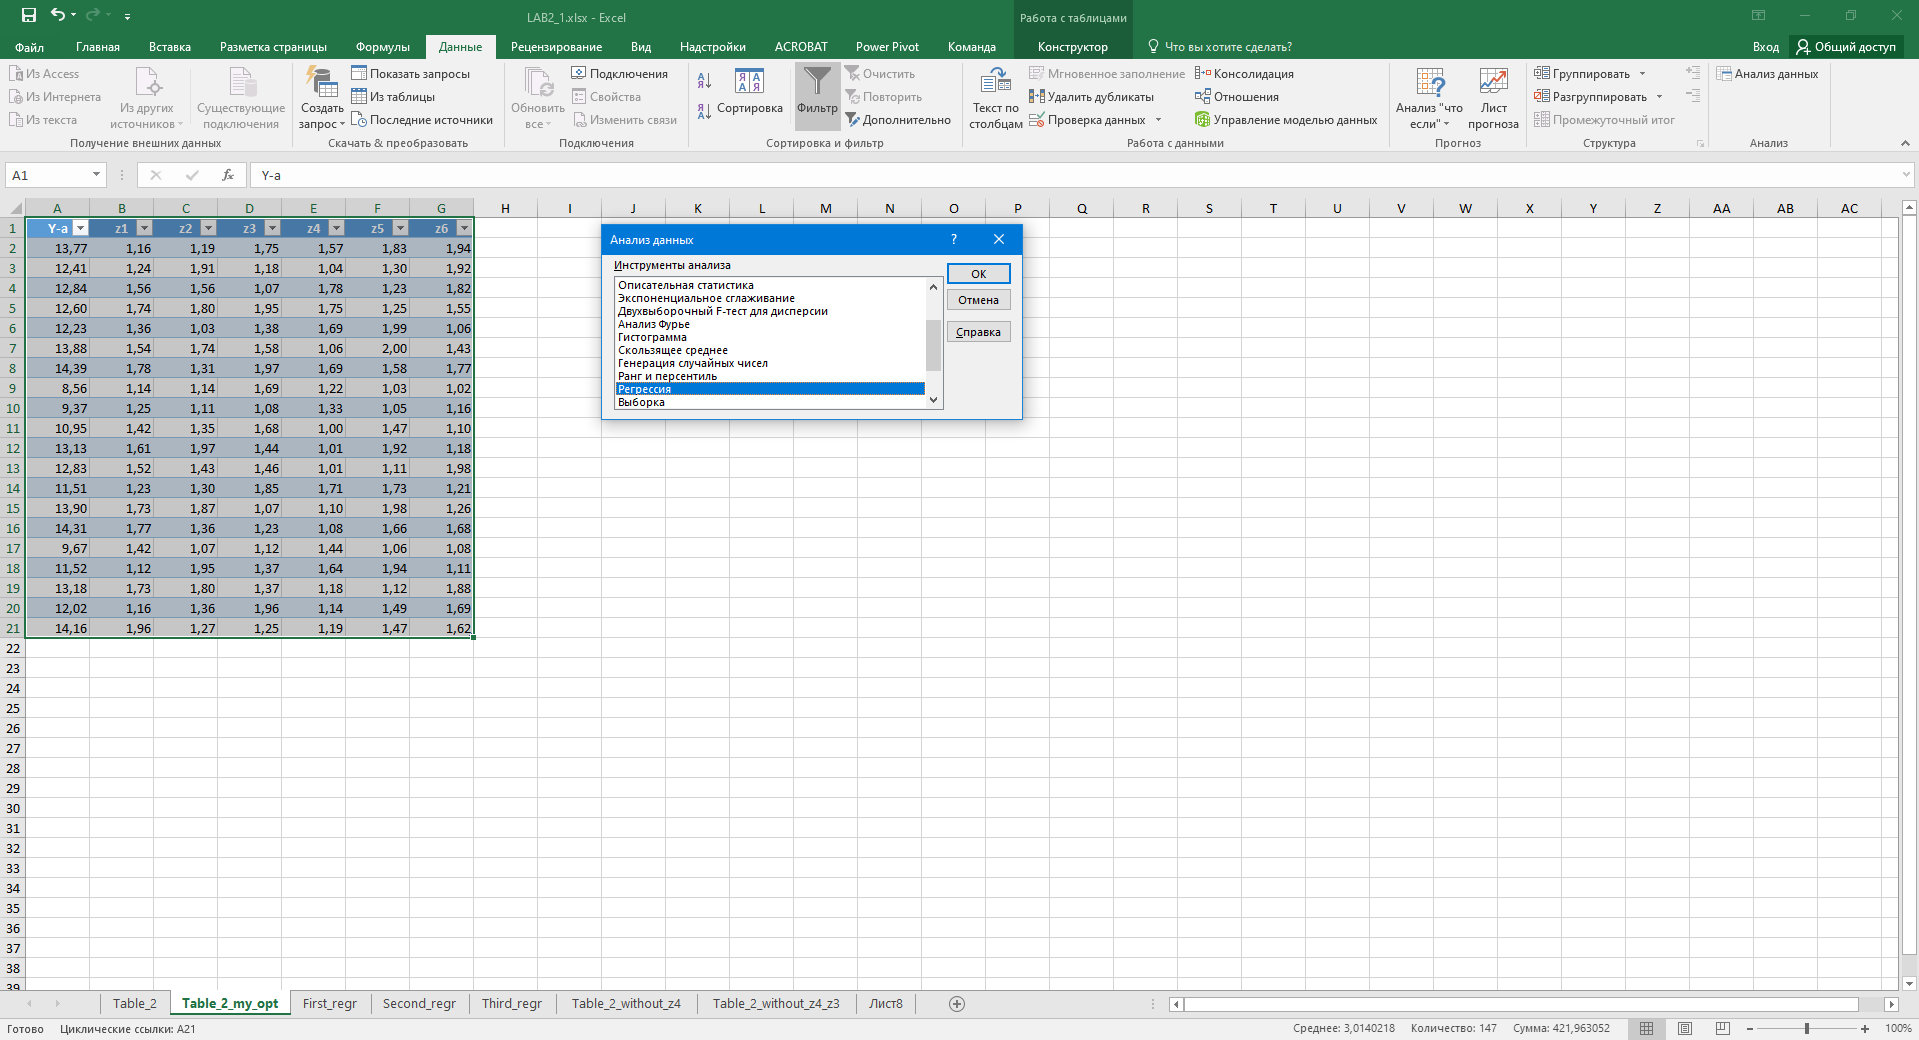
\includegraphics[width=1\linewidth]{../img1/first_screen.png}}
\end{figure}\\
В открывшемся окне заполняем поля, согласно следующему скриншоту, нажимаем <<ОК>>:
\begin{figure}[h]
	\center{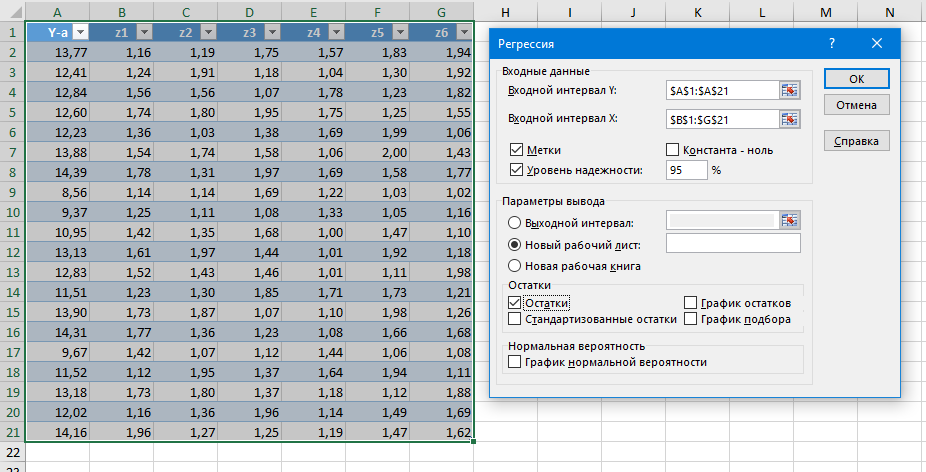
\includegraphics[width=1\linewidth]{../img1/second_screen.png}}
\end{figure}
\newpage
На новом листе видим результат первой регрессии. Обратим внимание на строки $16:23$. Для исключения незначимых параметров, найдём строки, в которых $|t-\textup{статистика}| < 2$. Выберем минимальное значение. В данном случае -- это строчка $21$, соответствующая $z4$.
\begin{figure}[h]
	\center{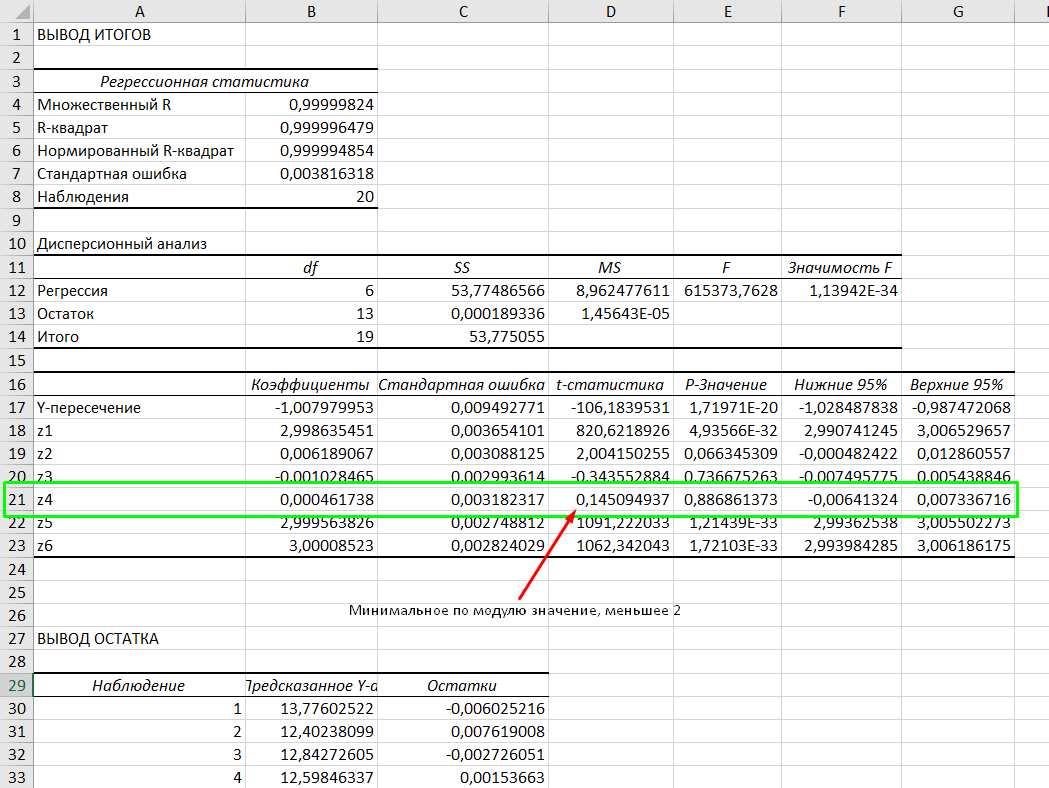
\includegraphics[width=1\linewidth]{../img1/first_regr.png}}
\end{figure}

\newpage
Исключая из исходной таблицы столбец, соответствующий $z4$ получим новую таблицу:
\begin{table}[htbp]
	\centering
	\caption{}
	\resizebox{!}{110pt}{
	\begin{tabular}{|rrrrrr|}
		\hline
		\rowcolor[rgb]{ .357,  .608,  .835} \multicolumn{1}{|c}{\textcolor[rgb]{ 1,  1,  1}{\textbf{Y-a}}} & \multicolumn{1}{c}{\textcolor[rgb]{ 1,  1,  1}{\textbf{z1}}} & \multicolumn{1}{c}{\textcolor[rgb]{ 1,  1,  1}{\textbf{z2}}} & \multicolumn{1}{c}{\textcolor[rgb]{ 1,  1,  1}{\textbf{z3}}} & \multicolumn{1}{c}{\textcolor[rgb]{ 1,  1,  1}{\textbf{z5}}} & \multicolumn{1}{c|}{\textcolor[rgb]{ 1,  1,  1}{\textbf{z6}}} \bigstrut\\
		\hline
		\rowcolor[rgb]{ .867,  .922,  .969} 13,77 & 1,16  & 1,19  & 1,75  & 1,83  & 1,94 \bigstrut\\
		\hline
		12,41 & 1,24  & 1,91  & 1,18  & 1,30  & 1,92 \bigstrut\\
		\hline
		\rowcolor[rgb]{ .867,  .922,  .969} 12,84 & 1,56  & 1,56  & 1,07  & 1,23  & 1,82 \bigstrut\\
		\hline
		12,60 & 1,74  & 1,80  & 1,95  & 1,25  & 1,55 \bigstrut\\
		\hline
		\rowcolor[rgb]{ .867,  .922,  .969} 12,23 & 1,36  & 1,03  & 1,38  & 1,99  & 1,06 \bigstrut\\
		\hline
		13,88 & 1,54  & 1,74  & 1,58  & 2,00  & 1,43 \bigstrut\\
		\hline
		\rowcolor[rgb]{ .867,  .922,  .969} 14,39 & 1,78  & 1,31  & 1,97  & 1,58  & 1,77 \bigstrut\\
		\hline
		8,56  & 1,14  & 1,14  & 1,69  & 1,03  & 1,02 \bigstrut\\
		\hline
		\rowcolor[rgb]{ .867,  .922,  .969} 9,37  & 1,25  & 1,11  & 1,08  & 1,05  & 1,16 \bigstrut\\
		\hline
		10,95 & 1,42  & 1,35  & 1,68  & 1,47  & 1,10 \bigstrut\\
		\hline
		\rowcolor[rgb]{ .867,  .922,  .969} 13,13 & 1,61  & 1,97  & 1,44  & 1,92  & 1,18 \bigstrut\\
		\hline
		12,83 & 1,52  & 1,43  & 1,46  & 1,11  & 1,98 \bigstrut\\
		\hline
		\rowcolor[rgb]{ .867,  .922,  .969} 11,51 & 1,23  & 1,30  & 1,85  & 1,73  & 1,21 \bigstrut\\
		\hline
		13,90 & 1,73  & 1,87  & 1,07  & 1,98  & 1,26 \bigstrut\\
		\hline
		\rowcolor[rgb]{ .867,  .922,  .969} 14,31 & 1,77  & 1,36  & 1,23  & 1,66  & 1,68 \bigstrut\\
		\hline
		9,67  & 1,42  & 1,07  & 1,12  & 1,06  & 1,08 \bigstrut\\
		\hline
		\rowcolor[rgb]{ .867,  .922,  .969} 11,52 & 1,12  & 1,95  & 1,37  & 1,94  & 1,11 \bigstrut\\
		\hline
		13,18 & 1,73  & 1,80  & 1,37  & 1,12  & 1,88 \bigstrut\\
		\hline
		\rowcolor[rgb]{ .867,  .922,  .969} 12,02 & 1,16  & 1,36  & 1,96  & 1,49  & 1,69 \bigstrut\\
		\hline
		14,16 & 1,96  & 1,27  & 1,25  & 1,47  & 1,62 \bigstrut\\
		\hline
	\end{tabular}}%
	\label{tab:addlabel2}%
\end{table}%
\\
Выполняя новую регрессию с аналогичными параметрами, получаем:
\begin{figure}[h]
	\center{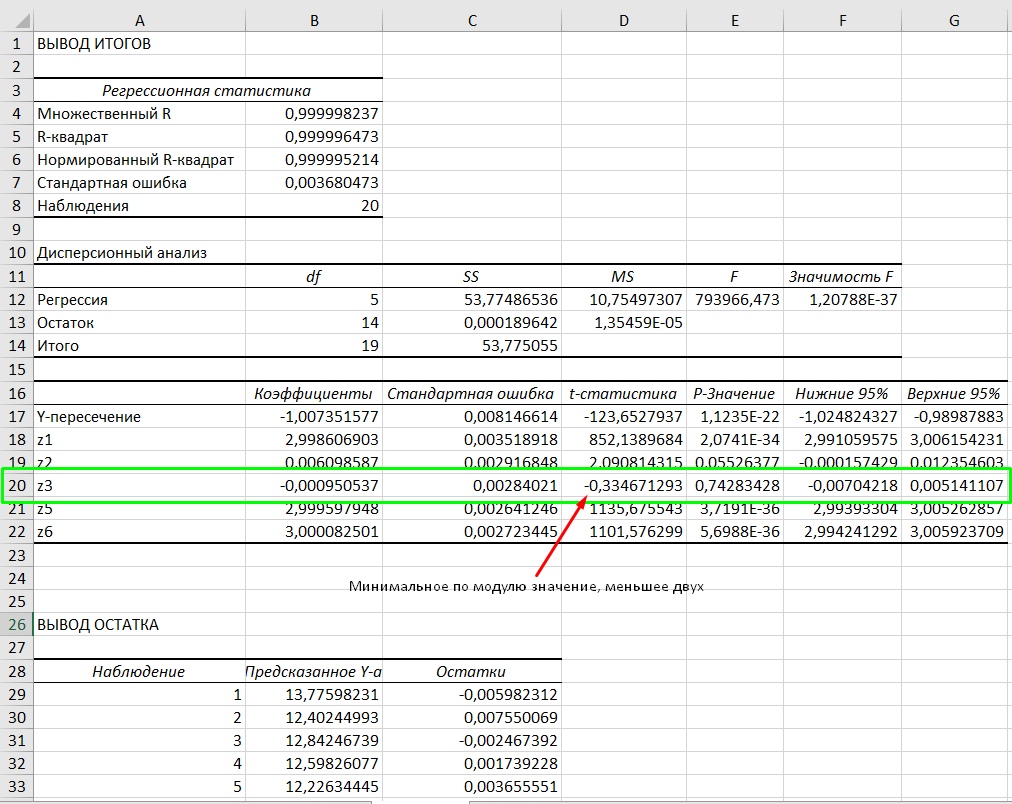
\includegraphics[width=.71\linewidth]{../img1/second_regr.png}}
\end{figure}
\\
В данном случае, незначимым параметром оказался параметр $z3$. Проделаем аналогичную процедуру: исключим $z3$ из Таблицы 2 и выполним для полученной таблицы регрессию.
\newpage

\begin{table}[htbp]
	\centering
	\caption{}
	\resizebox{!}{110pt}{
	\begin{tabular}{|rrrrr|}
		\hline
		\rowcolor[rgb]{ .357,  .608,  .835} \multicolumn{1}{|c}{\textcolor[rgb]{ 1,  1,  1}{\textbf{Y-a}}} & \multicolumn{1}{c}{\textcolor[rgb]{ 1,  1,  1}{\textbf{z1}}} & \multicolumn{1}{c}{\textcolor[rgb]{ 1,  1,  1}{\textbf{z2}}} & \multicolumn{1}{c}{\textcolor[rgb]{ 1,  1,  1}{\textbf{z5}}} & \multicolumn{1}{c|}{\textcolor[rgb]{ 1,  1,  1}{\textbf{z6}}} \bigstrut\\
		\hline
		\rowcolor[rgb]{ .867,  .922,  .969} 13,77 & 1,16  & 1,19  & 1,83  & 1,94 \bigstrut\\
		\hline
		12,41 & 1,24  & 1,91  & 1,30  & 1,92 \bigstrut\\
		\hline
		\rowcolor[rgb]{ .867,  .922,  .969} 12,84 & 1,56  & 1,56  & 1,23  & 1,82 \bigstrut\\
		\hline
		12,60 & 1,74  & 1,80  & 1,25  & 1,55 \bigstrut\\
		\hline
		\rowcolor[rgb]{ .867,  .922,  .969} 12,23 & 1,36  & 1,03  & 1,99  & 1,06 \bigstrut\\
		\hline
		13,88 & 1,54  & 1,74  & 2,00  & 1,43 \bigstrut\\
		\hline
		\rowcolor[rgb]{ .867,  .922,  .969} 14,39 & 1,78  & 1,31  & 1,58  & 1,77 \bigstrut\\
		\hline
		8,56  & 1,14  & 1,14  & 1,03  & 1,02 \bigstrut\\
		\hline
		\rowcolor[rgb]{ .867,  .922,  .969} 9,37  & 1,25  & 1,11  & 1,05  & 1,16 \bigstrut\\
		\hline
		10,95 & 1,42  & 1,35  & 1,47  & 1,10 \bigstrut\\
		\hline
		\rowcolor[rgb]{ .867,  .922,  .969} 13,13 & 1,61  & 1,97  & 1,92  & 1,18 \bigstrut\\
		\hline
		12,83 & 1,52  & 1,43  & 1,11  & 1,98 \bigstrut\\
		\hline
		\rowcolor[rgb]{ .867,  .922,  .969} 11,51 & 1,23  & 1,30  & 1,73  & 1,21 \bigstrut\\
		\hline
		13,90 & 1,73  & 1,87  & 1,98  & 1,26 \bigstrut\\
		\hline
		\rowcolor[rgb]{ .867,  .922,  .969} 14,31 & 1,77  & 1,36  & 1,66  & 1,68 \bigstrut\\
		\hline
		9,67  & 1,42  & 1,07  & 1,06  & 1,08 \bigstrut\\
		\hline
		\rowcolor[rgb]{ .867,  .922,  .969} 11,52 & 1,12  & 1,95  & 1,94  & 1,11 \bigstrut\\
		\hline
		13,18 & 1,73  & 1,80  & 1,12  & 1,88 \bigstrut\\
		\hline
		\rowcolor[rgb]{ .867,  .922,  .969} 12,02 & 1,16  & 1,36  & 1,49  & 1,69 \bigstrut\\
		\hline
		14,16 & 1,96  & 1,27  & 1,47  & 1,62 \bigstrut\\
		\hline
	\end{tabular}}%
	\label{tab:addlabel3}%
\end{table}%

\begin{figure}[h]
	\center{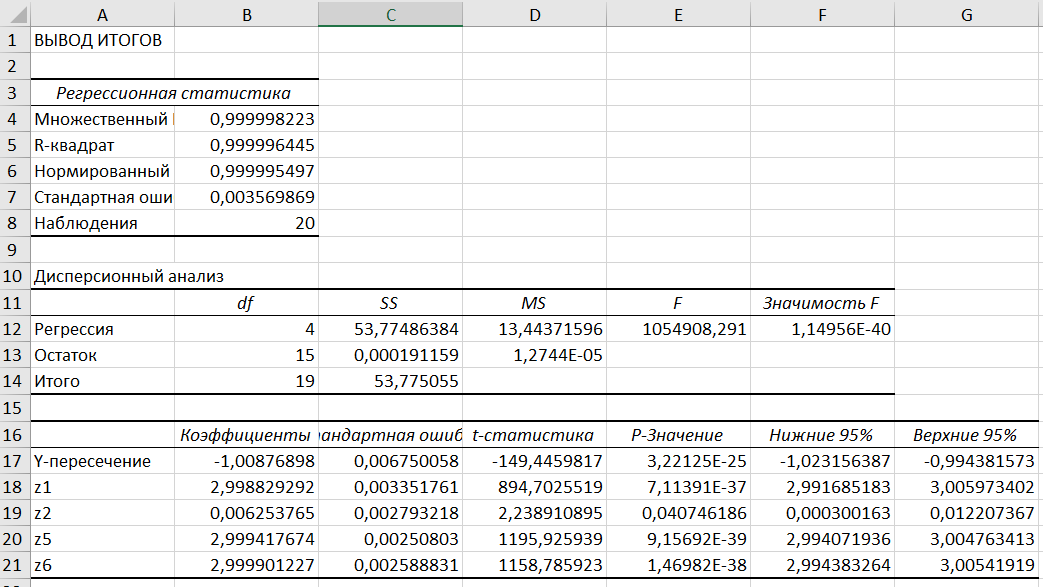
\includegraphics[width=1\linewidth]{../img1/third_regr.png}}
\end{figure}

Мы видим, что на данном шаге уже нет значений, для которых минимум модуля $t-$статистики превышал бы $2$. Значит полученные параметры являются значимыми. Оценка $\sigma$ соответствует значению <<Стандартная ошибка>> из ячейки $B7$, то есть $\hat{\sigma} = 0.003569869$.\\
Кроме того, отталкиваясь от значений коэффициентов, находящихся в ячейках $B17:B21$, можем выписать явное выражение:
\begin{equation*}
Y = -1.00876898 + 2.998829292 x_*^1 + 0.006253765 x_*^2 + 2.999417674 x_*^5 + 2.999901227 x_*^6
\end{equation*}

На листе с последней регрессией спустимся ниже и обнаружим таблицу <<Вывод остатка>>. Отталкиваясь от неё и от изначальных данных $y-\alpha$ построим график:

\begin{figure}[h]
	\center{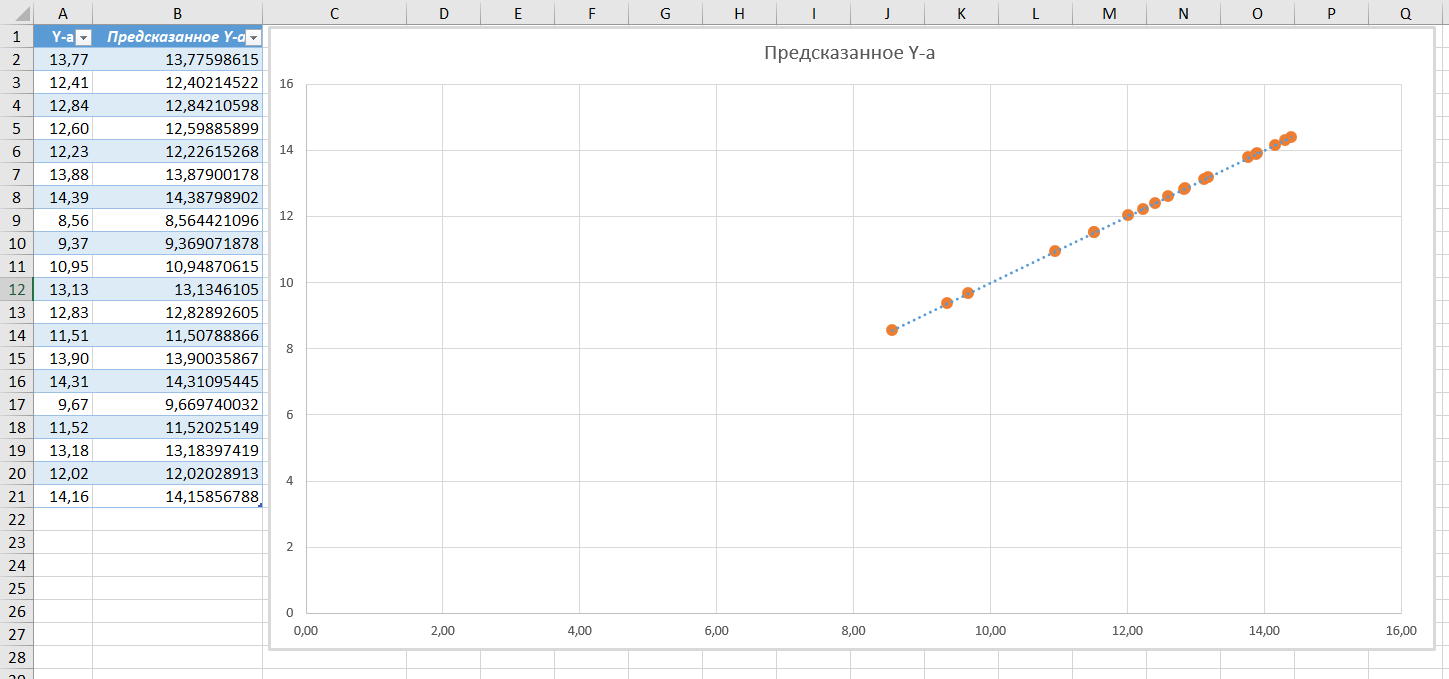
\includegraphics[width=1\linewidth]{../img1/graph.png}}
\end{figure}

\newpage
\section*{Задание 2.2}
\textbf{Задание.}Дана модель полиномиальной (кубической) регрессии:
\begin{equation}\label{eq2} 
	Y=x_{*}^{0}+t x_{*}^{1}+t^2 x_{*}^{2}+t^3 x_{*}^{3}+\varepsilon
\end{equation}
Для оценки неизвестных вектора тренда $\prescript{>}{}{x}_* = [x_*^0, x_*^1, x_*^2, x_*^3 \rangle \in \prescript{>}{}{\mathbb{E}}^{4}$ и параметра $\sigma$ случайной составляющей $\varepsilon \sim N(0, \sigma)$ модели линейной регрессии \ref{eq2} проводился эксперимент, в котором получены $m=20$ значений $y^1, \dots, y^m \in \mathbb{R}$ регрессора модели \ref{eq2} для $m$ попарно различных значений $t_1, \cdots, t_m \in \mathbb{R}$ единственного фактора модели \ref{eq2}.\\
Требуется получить оценки вектора тренда $\prescript{>}{}{x}_* = [x_*^0, x_*^1, x_*^2, x_*^3 \rangle \in \prescript{>}{}{\mathbb{E}}^{4}$ и параметра $\sigma$ случайной составляющей $\varepsilon \sim N(0, \sigma)$ модели полиномиальной (кубической) регрессии \ref{eq2}. Результаты расчётов проиллюстрировать графически, сопроводив необходимыми комментариями.\\
\textbf{Исходные данные.}\\
$N = 9$\\
$\alpha = 1$
\begin{table}[htbp]
	\centering
	\caption{}
	\resizebox{!}{180pt}{
	\begin{tabular}{|cccc|}
		\hline
		\rowcolor[rgb]{ .357,  .608,  .835} \multicolumn{1}{|l}{\textcolor[rgb]{ 1,  1,  1}{\textbf{$Y$}}} & \multicolumn{1}{l}{\textcolor[rgb]{ 1,  1,  1}{\textbf{$t_1$}}} & \multicolumn{1}{l}{\textcolor[rgb]{ 1,  1,  1}{\textbf{$t_1^2$}}} & \multicolumn{1}{l|}{\textcolor[rgb]{ 1,  1,  1}{\textbf{$t_1^3$}}} \bigstrut\\
		\hline
		\rowcolor[rgb]{ .867,  .922,  .969} -5,75 & 0,05  & 0,0025 & 0,00013 \bigstrut\\
		\hline
		-5,56 & 0,1   & 0,01  & 0,001 \bigstrut\\
		\hline
		\rowcolor[rgb]{ .867,  .922,  .969} -5,34 & 0,15  & 0,0225 & 0,00338 \bigstrut\\
		\hline
		-5,17 & 0,2   & 0,04  & 0,008 \bigstrut\\
		\hline
		\rowcolor[rgb]{ .867,  .922,  .969} -4,98 & 0,25  & 0,0625 & 0,01563 \bigstrut\\
		\hline
		-4,82 & 0,3   & 0,09  & 0,027 \bigstrut\\
		\hline
		\rowcolor[rgb]{ .867,  .922,  .969} -4,65 & 0,35  & 0,1225 & 0,04288 \bigstrut\\
		\hline
		-4,48 & 0,4   & 0,16  & 0,064 \bigstrut\\
		\hline
		\rowcolor[rgb]{ .867,  .922,  .969} -4,31 & 0,45  & 0,2025 & 0,09113 \bigstrut\\
		\hline
		-4,13 & 0,5   & 0,25  & 0,125 \bigstrut\\
		\hline
		\rowcolor[rgb]{ .867,  .922,  .969} -3,93 & 0,55  & 0,3025 & 0,16638 \bigstrut\\
		\hline
		-3,72 & 0,6   & 0,36  & 0,216 \bigstrut\\
		\hline
		\rowcolor[rgb]{ .867,  .922,  .969} -3,49 & 0,65  & 0,4225 & 0,27463 \bigstrut\\
		\hline
		-3,24 & 0,7   & 0,49  & 0,343 \bigstrut\\
		\hline
		\rowcolor[rgb]{ .867,  .922,  .969} -2,95 & 0,75  & 0,5625 & 0,42188 \bigstrut\\
		\hline
		-2,64 & 0,8   & 0,64  & 0,512 \bigstrut\\
		\hline
		\rowcolor[rgb]{ .867,  .922,  .969} -2,29 & 0,85  & 0,7225 & 0,61413 \bigstrut\\
		\hline
		-1,91 & 0,9   & 0,81  & 0,729 \bigstrut\\
		\hline
		\rowcolor[rgb]{ .867,  .922,  .969} -1,48 & 0,95  & 0,9025 & 0,85738 \bigstrut\\
		\hline
		-1    & 1     & 1     & 1 \bigstrut\\
		\hline
\end{tabular}}%
	\label{tab:addlabel4}%
\end{table}%
\newpage
\textbf{Решение.}\\
Для получения оценки вектора тренда  $\prescript{>}{}{x}_* = [x_*^0, x_*^1, x_*^2, x_*^3 \rangle \in \prescript{>}{}{\mathbb{E}}^{4}$ и параметра $\sigma$ случайной составляющей $\varepsilon \sim N(0, \sigma)$ модели полиномиальной (кубической) регрессии \ref{eq2} воспользуемся, аналогично первой части задания, программой <<Анализ данных>>, входящей в состав Excel. Переходя на вкладку <<Данные>>, выбираем программу <<анализ данных>>, в которой выбираем пункт <<регрессия>>.\\
Выставляя параметры регрессии, аналогичные предыдущей части задания, получим:
\begin{figure}[h]
	\center{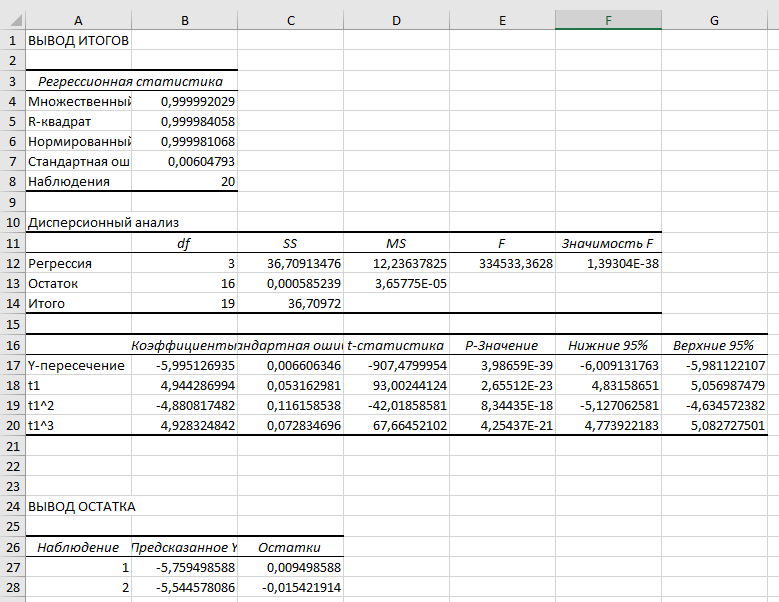
\includegraphics[width=1\linewidth]{../img2/first_screen.png}}
\end{figure}\\
Отметим, что все параметры полученной модели значимые.\\
Оценка $\sigma$ соответствует значению <<Стандартная ошибка>> из ячейки $B7$, то есть $\hat{\sigma} = 0.00604793
$.\\
Кроме того, отталкиваясь от значений коэффициентов, находящихся в ячейках $B17:B2$, можем выписать явное выражение:
\begin{equation*}
Y = -5.995126935 + 4.94428699432064 t - 4.88081748197511 t^2 + 4.92832484217597 t^3
\end{equation*}
\newpage
Отталкиваясь от полученных <<Предсказанных $Y$>> и изначальных данных график:
\begin{figure}[h]
	\center{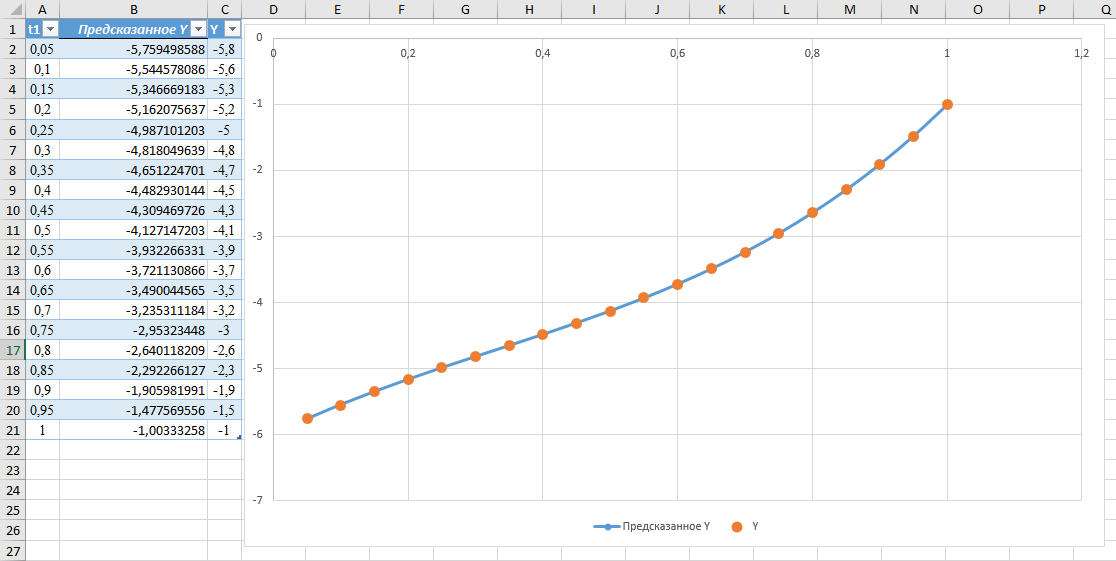
\includegraphics[width=1\linewidth]{../img2/graph.png}}
\end{figure}\\


\end{document}